\subsection{Đề 01}
\caulc
\Opensolutionfile{ans}[ans/ans-OTHKI-DE1-LC]
\begin{ex}%[0D3N2-4]
\immini{Cho hàm số $y=ax^2+bx+c$  có đồ thị $(P)$ như hình vẽ. Khẳng định nào sau đây là \textbf{sai}?
\choice
{Hàm số đồng biến trên khoảng $(-\infty;3)$}
{$(P)$ có đỉnh là $I(3;4)$}
{\True $(P)$ cắt trục tung tại điểm có tung độ bằng $4$}
{$(P)$ cắt trục hoành tại hai điểm phân biệt}}
{
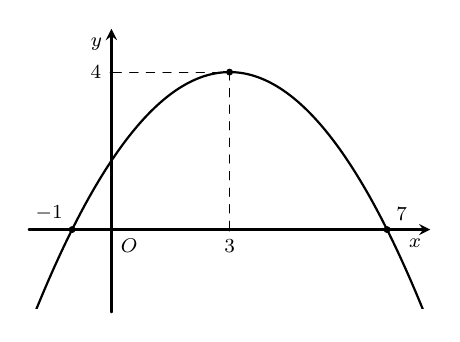
\begin{tikzpicture}[scale=0.5,line join=round,font=\footnotesize ,line cap=round,>=stealth,thick]
\tikzset{every node/.style={scale=0.9}}
\draw[->] (-2.1,0)--(8.1,0) node[below left] {$x$};
\draw[->] (0,-2.1)--(0,5.1) node[below left] {$y$};
\draw (0,0) node [below right] {$O$};
\foreach \x/\nx in {3/3}
\draw[thin] (\x,1pt)--(\x,-1pt) node [below] {$\nx$};
\foreach \y/\ny in {4/4}
\draw[thin]  (1pt,\y)--(-1pt,\y) node [left] {$\ny$};
\draw[dashed,thin](3,0)--(3,4)--(0,4);
\begin{scope}
\clip (-2,-2) rectangle (8,5);
\draw[samples=200,domain=-2:8,smooth,variable=\x] plot (\x,{-0.25*(\x)^2+1.5*(\x)+1.75});
\path (-1,0)node[above left]{$-1$};
\path (7,0)node[above right]{$7$};
\end{scope}
\fill (3,4)circle (2.5pt);
\fill (-1,0)circle (2.5pt);
\fill (7,0)circle (2.5pt);
\end{tikzpicture}
}
\loigiai{
Dựa vào đồ thị ta thấy $(P)$ cắt trục tung tại điểm có tung độ $y<4$.
}
\end{ex}

\begin{ex}%[0D3N2-1]
Trục đối xứng của parabol $(P)\colon y=2x^2+6x+3$  là
\choice
{\True $x=-\dfrac{3}{2}$}
{$x=-\dfrac{2}{3}$}
{$x=-3$}
{$y=-3$}
\loigiai{
Trục đối xứng $x=-\dfrac{b}{2a}=-\dfrac{6}{2\cdot2}=-\dfrac{3}{2}$.
}
\end{ex}

\begin{ex}%[0H5N1-1]
Cho tam giác $ABC$.  Có bao nhiêu vectơ khác vectơ-không có điểm đầu và điểm cuối là các đỉnh $A$, $B$, $C$?
\choice
{$3$} 
{\True $6$} 
{$4$} 
{$9$} 
\loigiai{
Các vectơ khác vectơ-không có điểm đầu và điểm cuối là các đỉnh $A$, $B$, $C$ là $\vv{AB}$, $\vv{BA}$, $\vv{AC}$, $\vv{CA}$, $\vv{BC}$, $\vv{CB}$.\\
Vậy có $6$ vectơ thỏa yêu cầu đề bài.
}
\end{ex}

\begin{ex}%[0H5N2-2]
Cho ba điểm phân biệt $A$, $B$, $C$.  Mệnh đề nào sau đây \textbf{đúng}?
\choice
{$AB+BC=AC$}
{\True $\vv{AB}+\vv{BC}+\vv{CA}=\vv{0}$}
{$\vv{AB}+\vv{AC}=\vv{BC}$}
{$\vv{AB}-\vv{BC}=\vv{AC}$}
\loigiai{
Ta có $\vv{AB}+\vv{BC}+\vv{CA}=\vv{AC}+\vv{CA}=\vv{AA}=\vv{0}$.
}
\end{ex}

\begin{ex}%[0H5N3-1]
Cho tam giác $ABC$.  Gọi $M$ và $N$ lần lượt là trung điểm của $AB$  và $AC$.  Khẳng định nào sau đây \textbf{sai}? 
\choice
{$\vv{AB}=2\vv{AM}$}
{$\vv{AC}=2\vv{NC}$}
{\True $\vv{BC}=-2\vv{MN}$}
{$\vv{CN}=-\dfrac{1}{2}\vv{AC}$}
\loigiai{
\immini{Ta có $MN$ là đường trung bình của tam giác $ABC$ \\ $\Rightarrow\heva{&MN\parallel BC\\&BC=2MN.}$\\
Mặt khác $\vv{MN}$ và $\vv{BC}$ là hai vectơ cùng chiều.\\
Do đó $\vv{BC}=2\vv{MN}$.}
{
\begin{tikzpicture}[scale=1,line join=round,font=\footnotesize ,line cap=round,thick]
\coordinate (A) at (-0.5,3);
\coordinate (B) at (-2,0);
\coordinate (C) at (2.5,0);
\path ($(A)!0.5!(B)$) coordinate (M) ;
\path ($(A)!0.5!(C)$) coordinate (N) ;
\draw(A)--(B)--(C)--cycle (M)--(N);
\foreach \i/\g in {A/90,B/-90,C/-90,M/180,N/0}{\draw[fill=black](\i) circle (1pt) ($(\i)+(\g:3mm)$) node[scale=1]{$\i$};}
\end{tikzpicture}
}
}
\end{ex}

\begin{ex}%[0H5N4-4]
Cho tam giác $ABC$ vuông cân tại $A$ và $AB=1$. Khẳng định nào sau đây \textbf{sai}?
\choice
{$\vv{BA}\cdot \vv{BC}=1$}
{$\vv{CA}\cdot \vv{CB}=1$}
{\True $\vv{AB}\cdot \vv{AC}=1$}
{$\vv{AB}\cdot \vv{BC}=-1$}
\loigiai{
\begin{center}
\begin{tikzpicture}[scale=1,line join=round,font=\footnotesize ,line cap=round,thick]
	\coordinate (B) at (-2,0);
	\coordinate (C) at (2.25,0);
	\coordinate (Temp) at ($(B) + (45:1)$);
	\coordinate (A) at ($(B)!(C)!(Temp)$);
	\path ($(A)!0.5!(B)$) node [left]{$1$};
	\draw(A)--(B)--(C)--cycle;
	\pic[draw,thin,angle radius=2mm] {right angle = B--A--C};
	\foreach \i/\g in {A/90,B/-90,C/-90}{\draw[fill=white](\i) circle (1pt) ($(\i)+(\g:3mm)$) node[scale=1]{$\i$};}
\end{tikzpicture}
\end{center}
\begin{enumerate}[$\bullet$]
\allowdisplaybreaks
\item Xét $\vv{BA}\cdot \vv{BC}$.
\begin{align*}
	\vv{BA}\cdot \vv{BC}&=\left|\vv{BA} \right|\cdot\left|\vv{BC} \right|\cdot\cos\left(\vv{BA},\vv{BC} \right)\\
	&=1\cdot \sqrt{2}\cdot \cos 45^\circ=1.
\end{align*}
\item Xét $\vv{CA}\cdot \vv{CB}$.
\begin{align*}
	\vv{CA}\cdot \vv{CB}&=\left|\vv{CA} \right|\cdot\left|\vv{CB} \right|\cdot\cos\left(\vv{CA},\vv{CB} \right)\\
	&=1\cdot \sqrt{2}\cdot \cos 45^\circ=1.
\end{align*}
\item Xét $\vv{AB}\cdot \vv{AC}$.\\
Do tam giác $ABC$ vuông cân tại $A$ nên $AB\perp AC\Rightarrow \vv{AB}\cdot \vv{AC}=0$.
\item Xét $\vv{AB}\cdot \vv{BC}$.
\begin{align*}
	\vv{AB}\cdot \vv{BC}&=-\vv{BA}\cdot \vv{BC}\\
	&=-\left|\vv{BA}\right|\cdot\left|\vv{BC} \right|\cdot\cos\left(\vv{BA},\vv{BC} \right)\\
	&=-1\cdot \sqrt{2}\cdot \cos 45^\circ=-1.
\end{align*}
\end{enumerate}
}
\end{ex}

\begin{ex}%[0H5H4-1]
Cho tam giác $ABC$ vuông tại $A$ có $\widehat{B}=30^\circ$, $AC=2$.  Gọi $M$ là trung điểm của $BC$. Giá trị của biểu thức $P=\vv{AM}\cdot \vv{BM}$ bằng
\choice
{\True $-2$} 
{$2\sqrt{3}$} 
{ $2$} 
{$-2\sqrt{3}$} 
\loigiai{
\begin{center}
\begin{tikzpicture}[scale=1,line join=round,font=\footnotesize ,line cap=round,thick]
	\coordinate (B) at (-3,0);
	\coordinate (C) at (2,0);
	\coordinate (Temp) at ($(B) + (30:1)$);
	\coordinate (A) at ($(B)!(C)!(Temp)$);
	\path ($(B)!0.5!(C)$) coordinate (M);
	\path ($(A)!0.5!(C)$)node [above right]{$2$};
	\draw(A)--(B)--(C)--cycle (A)--(M);
	\pic[draw,thin,angle radius=2mm] {right angle = B--A--C};
	\foreach \i/\g in {A/90,B/-90,C/-90,M/-90}{\draw[fill=black](\i) circle (1pt) ($(\i)+(\g:3mm)$) node[scale=1]{$\i$};}
	\pic["$30^\circ$",draw,angle radius=5mm,angle eccentricity=1.6]{angle=C--B--A};
\end{tikzpicture}	
\end{center}
Xét tam giác $ABC$ vuông tại $A$ có $\widehat{B}=30^\circ\Rightarrow \widehat{C}=60^\circ$.\\
Mặt khác $M$ là trung điểm của $BC$ nên $AM=MC=\dfrac{BC}{2}$.\\
Do đó tam giác $MAC$ đều $\Rightarrow MA=MC=AC=2$.\\
Khi đó 
\begin{align*}
P=\vv{AM}\cdot \vv{BM}&=\vv{AM}\cdot \vv{MC}\\
&=-\vv{MA}\cdot \vv{MC}\\
&=-\left|\vv{MA} \right|\cdot \left|\vv{MC}\right|\cdot \cos \left(\vv{MA},\vv{MC}\right)\\
&=-2\cdot 2\cdot \cos 60^\circ=-2.
\end{align*}
}
\end{ex}

\begin{ex}%[0D6N1-3]
Khi sử dụng máy tính bỏ túi với $10$ chữ số thập phân ta được $\sqrt{8}=2{,}828427125$. Giá trị gần đúng của $\sqrt{8}$ chính xác đến hàng phần trăm là
\choice
{$2{,}81$}
{\True $2{,}83$}
{$2{,}82$}
{$2{,}80$}
\loigiai{
Giá trị gần đúng của $\sqrt{8}=2{,}828427125$ chính xác đến hàng phần trăm là $2{,}83$.
}
\end{ex}

\begin{ex}%[0D6N2-3]
Tâm ghi lại số liệu từ trang web của Tổng cục thống kê bảng nhiệt độ không khí trung bình các tháng trong năm $2020$ tại một trạm quan trắc đặt ở thành phố Vinh.
\begin{longtable}{|c|c|c|c|c|c|c|c|c|c|c|c|c|}
\hline  
Tháng&$1$&$2$&$3$&$4$&$5$&$6$&$7$&$8$&$9$&$10$&$11$&$12$\\
\hline
Nhiệt độ&$20{,}9$&$20{,}7$&$23{,}7$&$23$&$29{,}5$&$32{,}2$&$4{,}5$&$29{,}6$&$28{,}9$&$23{,}8$&$23{,}1$&$18{,}4$\\
\hline
\end{longtable}\noindent
Bạn Tâm đã ghi nhầm nhiệt độ của một tháng trong bảng bên. Theo em bạn Tâm đã ghi nhầm số liệu của tháng mấy?
\choice
{Tháng $6$}
{\True Tháng $7$}
{Tháng $12$}
{Tháng $1$}
\loigiai{
Tâm ghi nhầm nhiệt độ của tháng $7$.\\
Do tháng $7$ là vào mùa hè nên nhiệt độ trung bình trong tháng đó ở thành phố Vinh phải cao hơn $4{,}5^\circ$.
}
\end{ex}

\begin{ex}%[0D6N3-3]
Cho dãy số liệu thống kê  $32, 33, 36, 38, 39, 42, 46$. Khi đó  trung vị là
\choice
{$32$}
{$46$}
{$37$}
{\True $38$}
\loigiai{
Mẫu số liệu sắp xếp theo thứ tự không giảm $32, 33, 36, 38, 39, 42, 46$.\\
Cỡ mẫu $n=7$ nên trung vị của mẫu số liệu là $M_e=x_4=38$.
}
\end{ex}

\begin{ex}%[0D6N4-4]
Theo kết quả thống kê điểm thi giữa kỳ $2$ môn toán khối $10$ của một trường THPT, người ta tính được phương sai của bảng thống kê đó là $S_x^2=0{,}573$. Độ lệch chuẩn của bảng thống kê đó bằng
\choice
{$0{,}812$}
{\True $0{,}757$}
{$0{,}936$}
{$0{,}657$}
\loigiai{
Độ lệch chuẩn $S_x=\sqrt{S_x^2}=\sqrt{0{,}573}\approx 0{,}757$.
}
\end{ex}

\begin{ex}%[0D6H4-4]
Bảng số liệu sau cho biết thời gian làm bài tính bằng phút của $50$ học sinh.
\begin{longtable}{|c|c|c|c|c|c|c|c|c|c|c|c|}
\hline
Thời gian&$3$&$4$&$5$&$6$&$7$&$8$&$9$&$10$&$11$&$12$&\\
\hline
Số học sinh&$1$&$3$&$4$&$7$&$8$&$9$&$8$&$5$&$3$&$2$&$N=50$\\
\hline
\end{longtable}
Phương sai của mẫu số liệu thống kê trên bằng
\choice
{$7{,}68$}
{$2{,}13$}
{$4{,}63$}
{\True $4{,}54$}
\loigiai{
Thời gian làm bài trung bình của $50$ học sinh
$$\overline{x}=\dfrac{1}{50}(3\cdot 1+4\cdot 3+5\cdot 4+6\cdot 7+7\cdot 8+8\cdot 9+9\cdot 8+10\cdot 5+11\cdot 3+12\cdot 2)= 7{,}68.$$
Phương sai của mẫu số liệu \\$S^2=\dfrac{1\cdot 3^2+3\cdot4^2+4\cdot5^2+7\cdot6^2+8\cdot7^2+9\cdot8^2+8\cdot9^2+5\cdot10^2+3\cdot11^2+2\cdot12^2}{50}-7{,}68^2$\\$\approx 4{,}54$.
}
\end{ex}
\Closesolutionfile{ans}
\indapan{6}{ans/ans-OTHKI-DE1-LC}
\Opensolutionfile{ans}[ans/ans-OTHKI-DE1-DS]
\cauds
\begin{ex}%[0H5N1-3]
Cho tam giác $ABC$. Gọi $M$, $N$, $P$ lần lượt là trung điểm của các cạnh $BC$, $CA$ và $AB$. Khi đó
\choiceTF
{\True $PN$ là đường trung bình của tam giác $ABC$}
{\True $\vv{PN}$, $\vv{MC}$ cùng hướng với vectơ $\vv{BM}$}
{$\vv{BM}=\vv{NP}$}
{\True $\vv{BM}$ có các vectơ đối là $\vv{NP}$, $\vv{CM}$, $\vv{MB}$}
\loigiai{
\begin{center}
\begin{tikzpicture}[scale=1,line join=round,font=\footnotesize ,line cap=round,thick]
\coordinate (A) at (0,3);
\coordinate (B) at (-2,0);
\coordinate (C) at (3,0);
\path ($(B)!0.5!(C)$) coordinate (M) ;
\path ($(A)!0.5!(C)$) coordinate (N) ;
\path ($(A)!0.5!(B)$) coordinate (P) ;
\draw(A)--(B)--(C)--cycle (M)--(N)--(P)--cycle;
\foreach \i/\g in {A/90,B/-90,C/-90,M/-90,N/45,P/120}{\draw[fill=black](\i) circle (1pt) ($(\i)+(\g:3mm)$) node[scale=1]{$\i$};}
\end{tikzpicture}
\begin{itemchoice}
\itemch{\bf Đúng.}\\
Ta có $N$, $P$ lần lượt là trung điểm của $AC$, $AB$ nên $PN$ là đường trung bình của tam giác $ABC$.
\itemch{\bf Đúng.}\\
Ta có $PN\parallel BM\parallel MC$ và ba vectơ này cùng chiều nên $\vv{PN}$, $\vv{MC}$ cùng hướng với vectơ $\vv{BM}$.
\itemch{\bf Sai.}\\
Do $\vv{PN}$ và $\vv{BM}$ cùng hướng nên $\vv{NP}$ và $\vv{BM}$ ngược hướng.\\
Do đó $\vv{BM}=-\vv{NP}$.
\itemch{\bf Đúng.}\\
$\vv{BM}$ có các vectơ đối là $\vv{NP}$, $\vv{CM}$, $\vv{MB}$.
\end{itemchoice}
\end{center}
}
\end{ex}

\begin{ex}%[0D3H2-2]
Cho hàm số $y=-x^2+3$ có đồ thị $(P)$. Khi đó
\choiceTF
{\True Tọa độ đỉnh của $(P)$ là $I(0;3)$}
{Bề lõm của $(P)$ hướng lên}
{Hàm số đã cho đồng biến trên khoảng $(0;+\infty)$ và nghịch biến trên khoảng $(-\infty;0)$}
{\True Giá trị lớn nhất của hàm số $y_{\max}=3$ khi $x=0$}
\loigiai{
\begin{itemchoice}
\itemch{\bf Đúng.}\\
Hoành độ đỉnh $x=-\dfrac{b}{2a}=-\dfrac{0}{-2}=0\Rightarrow y=-0^2+3=3$.\\
Tọa độ đỉnh $I(0;3)$.
\itemch{\bf Sai.}\\
Do $a=-1<0$ nên bề lõm  của $(P)$ hướng xuống.
\itemch{\bf Sai.}\\
Ta có bảng biến thiên
\begin{center}
	
\begin{tikzpicture}
		\tkzTabInit[espcl=2.5,lgt=1.5]
		{$x$/0.7,$y$/2.1}
		{$-\infty$,$0$,$+\infty$}
	%	\tkzTabLine{,+,0,-,}
		\tkzTabVar{-/$-\infty$,+/$3$,-/$-\infty$}
	\end{tikzpicture}
\end{center}
Từ bảng biên thiên ta thấy\\
Hàm số đã cho đồng biến trên khoảng $(-\infty;0)$ và nghịch biến trên khoảng $(0;+\infty)$
\itemch{\bf Đúng.}\\
Ta có bảng biến thiên
\begin{center}
	
\begin{tikzpicture}
		\tkzTabInit[espcl=2.5,lgt=1.5]
		{$x$/0.7,$y$/2.1}
		{$-\infty$,$0$,$+\infty$}
		%	\tkzTabLine{,+,0,-,}
		\tkzTabVar{-/$-\infty$,+/$3$,-/$-\infty$}
	\end{tikzpicture}
\end{center}
Từ bảng biên thiên ta thấy $y_{\max}=3$ khi $x=0$.
\end{itemchoice}
}
\end{ex}

\begin{ex}%[0H5H3-2]
Cho hình bình hành $ABCD$. Gọi $I$, $J$ lần lượt là trung điểm $BC$ và $CD$. Khi đó
\choiceTF
{\True $\vv{AC}=\vv{AB}+\vv{AD}$}
{$\vv{IJ}=\vv{AI}+\vv{AJ}$}
{$\vv{AI}=\vv{AB}+\dfrac{3}{2}\vv{AD}$}
{$\vv{AJ}=\dfrac{1}{2}\vv{AB}+\dfrac{1}{2}\vv{AD}$}
\loigiai{
\begin{center}
	\begin{tikzpicture}[scale=1,line join=round,font=\footnotesize ,line cap=round,thick]
		\coordinate (A) at (1,3);
		\coordinate (B) at (6,3);
		\coordinate (D) at (0,0);
		\coordinate (C) at ($(B)+(D)-(A)$);
		\path ($(B)!0.5!(C)$) coordinate (I) ;
		\path ($(C)!0.5!(D)$) coordinate (J) ;
		\draw(A)--(B)--(C)--(D)--cycle (A)--(I);
		\foreach \i/\g in {A/90,B/90,C/-90,D/-90,I/0,J/-90}{\draw[fill=black](\i) circle (1pt) ($(\i)+(\g:3mm)$) node[scale=1]{$\i$};}
	\end{tikzpicture}
\end{center}
\begin{itemchoice}
\itemch {\bf Đúng.}\\
Ta có $\vv{AB}+\vv{AD}=\vv{AC}$ (quy tắc hình bình hành).
\itemch {\bf Sai.}\\
Ta có $\vv{AJ}-\vv{AI}=\vv{IJ}$ (quy tắc ba điểm).
\itemch {\bf Sai.}\\
Ta có $\vv{AI}=\vv{AB}+\vv{BI}=\vv{AB}+\dfrac{1}{2}\vv{BC}=\vv{AB}+\dfrac{1}{2}\vv{AD}$. 
\itemch {\bf Sai.}\\
Ta có $\vv{AJ}=\dfrac{1}{2}(\vv{AD}+\vv{AC})=\dfrac{1}{2}(\vv{AD}+\vv{AD}+\vv{AB})=\vv{AD}+\dfrac{1}{2}\vv{AB}$. 
\end{itemchoice}
}
\end{ex}

\begin{ex}%[0D6H4-4]
Mẫu số liệu dưới đây thống kê thời gian chờ xe bus (đơn vi: phút) của $10$ học sinh ở cùng một bến: $1, 4, 5, 6, 6, 8, 10, 11, 12, 25$. Khi đó
\choiceTF
{\True Thời gian chờ xe bus trung bình của $10$ học sinh trên là $8{,}8$ phút}
{Mốt của mẫu số liệu trên bằng $25$}
{\True Giá trị ngoại lệ của mẫu số liệu trên là $25$}
{\True Độ lệch chuẩn về thời gian chờ xe bus của $10$ học sinh trên là $6{,}27$ phút}
\loigiai{
\begin{itemchoice}
\itemch{\bf Đúng.}\\
Thời gian chờ xe bus trung bình của $10$ học sinh trên là \[\overline{x}=\dfrac{1+4+5+6+6+8+10+11+12+25}{10}=8{,}8\,(\text{phút}).\]
\itemch{\bf Sai.}\\
Dựa vào mẫu số liệu ta thấy thời gian chờ xe bus $6$ phút có $2$ học sinh, những thời gian còn lại chỉ có $1$ học sinh.\\
Do đó mốt của mẫu số liệu là $M_0=6$.
\itemch{\bf Đúng.}\\
Sắp xếp mẫu số liệu theo thứ tự không giảm $1, 4, 5, 6, 6, 8, 10, 11, 12, 25$.\\
Cỡ mẫu $n=10$.\\
Tứ phân vị thứ nhất là $Q_1=x_3=5$.\\
Tứ phân vị thứ ba là $Q_3=x_8=11$.\\
Khoảng tứ phân vị $\Delta Q=Q_3-Q_1=11-5=6$.\\
Ta có $\Delta Q-1{,}5\cdot Q_1=6-1{,}5\cdot 5=-1{,}5$ và $\Delta Q+1{,}5\cdot Q_3=6+1{,}5\cdot 11=22{,}5$.\\
Ta thấy $25>22{,}5$ nên $25$ là giá trị ngoại lệ.
\itemch{\bf Đúng.}\\
Phương sai $S^2=\dfrac{1^2+4^2+5^2+6^2+6^2+8^2+10^2+11^2+12^2+25^2}{10}-8{,}8^2=39{,}36$.\\
Độ lệch chuẩn $S=\sqrt{S^2}=\sqrt{39{,}36}\approx 6{,27}$.
\end{itemchoice}
}
\end{ex}
\Closesolutionfile{ans}
\indapan{3}{ans/ans-OTHKI-DE1-DS}
\Opensolutionfile{ans}[ans/ans-OTHKI-DE1-KQ]
\caukq
\begin{ex}%[0D3V2-6]
\immini{Một viên bi được ném xiên từ vị trí $A$  cách mặt đất $2\mathrm{\,m}$ theo quỹ đạo dạng parabol như hình vẽ bên. Tìm khoảng cách từ vị trí $E$ đến vị trí $F$, biết vị trí $E$ là nơi viên bi rơi xuống chạm mặt đất (kết quả làm tròn đến số thập phân thứ hai).}
{
\begin{tikzpicture}[scale=1,line join=round,font=\footnotesize,line cap=round,>=stealth,yscale=0.7]
\draw[->] (0,0)--(3,0) node[below] {$x$};
\draw[->] (0,0)--(0,8) node[left] {$y$};
\draw (0,0) node [below left] {$O$};
\foreach \x/\nx in {1/1}
\draw[thin] (\x,1pt)--(\x,-1pt) node [below] {$\nx$};
\foreach \y/\ny in {2/2,3/3,4/4,5/5,6/6,7/7}
\draw[thin] (1pt,\y)--(-1pt,\y) node [left] {$\ny$};
\draw[dashed,thin](1,0)--(1,7)--(0,7);
\begin{scope}
\clip (-1,-1) rectangle (3,8);
\draw[samples=200,domain=0:2.183,smooth,variable=\x] plot (\x,{-5*(\x)^2+10*(\x)+2});
\path (0,2)node[right]{$A$};
\path (1,7)node[above]{$C$};
\path(2.183,0)node[below]{$E$};
\path(0,0)node[above right]{$F$};
\fill  (0,0)circle (1.5pt) (1,7)circle (1.5pt) (0,2)circle (1.5pt) (2.183,0)circle (1.5pt);
\end{scope}
\end{tikzpicture}
}
\shortans[6]{$2{,}18$}
\loigiai{
Đặt hệ trục tọa độ $Oxy$ sao cho điểm $F$ trùng với gốc tọa độ $O$ và điểm $A$ thuộc tia $Oy$, điểm $E$ thuộc tia $Ox$.\\
Gọi parabol có dạng $(P)\colon y=ax^2+bx+c\,(a\ne 0)$.\\
Ta có $A(0;2)\in (P)\Rightarrow c=2$.\\
Hoành độ đỉnh $x=-\dfrac{b}{2a}=1\Rightarrow 2a+b=0.\,(1)$\\
$C(1,7)\in (P)\Rightarrow a+b+c=7\Rightarrow a+b=5.\,(2)$\\
Từ $(1)$ và $(2)\Rightarrow a=-5, b=10$.\\
Vậy $(P)\colon y=-5x^2+10x+2$.\\
Ta có $E(x,0)\in (P)\Rightarrow -5x^2+10x+2=0\Rightarrow \hoac{&x=\dfrac{5+\sqrt{35}}{5}\\&x=\dfrac{5-\sqrt{35}}{5}.}$\\
Do $E$ thuộc tia $Ox$ nên $x>0\Rightarrow x=\dfrac{5+\sqrt{35}}{5}\approx 2{,}18$.\\
Vậy $EF\approx 2{,}18$.
}
\end{ex}

\begin{ex}%[0H4V3-2]
Trên nóc một tòa nhà có một cột ăng-ten cao $5\mathrm{\,m}$. Từ một vị trí quan sát $A$ cao $7\mathrm{\,m}$ so với mặt đất có thể nhìn thấy đỉnh $B$ và chân $C$ của cột ăng-ten, với các góc tương ứng là $50^\circ$ và $40^\circ$ so với phương nằm ngang (hình bên dưới). Tính chiều cao của tòa nhà (làm tròn kết quả đến hàng phần mười).
\begin{center}
\begin{tikzpicture}[scale=.6, font=\footnotesize, line join=round, >=stealth,thick]
\coordinate (O) at (0,0);
\def\nhathap{2} %so tang nha thap
\def\nhacao{5} %so tang nha cao
\def\kc{10} %khoang cach 2 nha
\def\dai{1} %chieu dai 1 khoi
\def\cao{2} %chieu cao 1 khoi
\coordinate (H) at (\kc,0);
\newcommand{\xaynha}[2]{
\draw[very thick] (#1,#2)rectangle(#1+\dai,#2+\cao);
\draw[very thick,fill=black] (#1,#2)rectangle(#1+\dai,#2+0.25*\cao);
\draw[very thick] (#1+0.2*\dai,#2+0.25*\cao)rectangle(#1+0.8*\dai,#2+0.9*\cao);
}
%Xay nha thap
\foreach \j in {1,...,\nhathap}{
\foreach \i in {0,...,4}{
\xaynha{\i*1.1}{\j*\cao}
}
}
\draw[line width=0.2cm] (-0.1,\cao*\nhathap+\cao)--(5*\dai*1.1,\cao*\nhathap+\cao);
\foreach \j in {1,...,\nhacao}{
\foreach \i in {0,...,4}{
\xaynha{\i*1.1+\kc}{\j*\cao}
}
}
\draw[line width=0.2cm] (-0.1+\kc,\cao*\nhacao+\cao)--(5*\dai*1.1+\kc,\cao*\nhacao+\cao);
\coordinate (A) at (5*\dai*1.1,\cao*\nhathap+\cao+0.1);
\draw (A) node[above left]{$A$};
\coordinate (C) at (\kc,\cao*\nhacao+\cao);
\draw (C) node[above right]{$C$};
\coordinate (B) at ($(C)+(0,2)$);
\draw (B) node[above]{$B$};
\coordinate (H) at (\kc,\cao);
\draw (H) node[below]{$H$};
\coordinate (D) at (\kc,\cao*\nhathap+\cao+0.1);
\draw (D) node[above left]{$D$};
\draw[very thick] (-0.5,\cao)--(\kc+5*\dai*1.2,\cao);
\draw [dashed](A)--(D); \draw (B)--(A)--(C);\draw[line width=0.07cm] (C)--(B);
\draw ($(B)+(135:0.5cm)$)--($(B)+(-45:0.5cm)$);
\pic["$40^\circ$",draw,angle radius=5mm,angle eccentricity=1.6]{angle=D--A--C};
\pic["$50^\circ$",draw,double,angle radius=12mm,angle eccentricity=1.3]{angle=D--A--B};
\path ($(C)!0.55!(B)$) node [right]{$5\mathrm{\,m}$};
\path ($(D)!0.5!(H)$) node [left]{$7\mathrm{\,m}$};
\end{tikzpicture}
\end{center}
\shortans[6]{$18{,}9$}
\loigiai{
Xét tam giác $ABC$, ta có $\widehat{A}=50^\circ-40^\circ=10^\circ$.\\
Ta có tam giác $ABD$ vuông tại $D$ nên $\widehat{B}=90^\circ-50^\circ=40^\circ$.\\
Áp dụng định lí sin trong tam giác $ABC$, ta có $AC=b=\dfrac{a\cdot \sin B}{\sin A}=\dfrac{5\cdot \sin 40^\circ}{\sin 10^\circ}\approx 18{,}5\mathrm{\,cm}$.\\
Xét tam giác $ACD$ vuông tại $D$, ta có $CD=AC\cdot \sin A=18{,}5\cdot \sin 40^\circ\approx 11{,}9\mathrm{\,cm}$.\\
Vậy chiều cao tòa nhà $CH=CD+DH\approx 11{,}9+7\approx 18{,}9\mathrm{\,cm}$. 

}
\end{ex}

\begin{ex}%[0H5V2-6]
Một dòng sông chảy từ phía Bắc xuống phía Nam với vận tốc $10\mathrm{\,km/h}$, có một chiếc ca nô 
chuyển động từ phía Đông sang phía Tây với vận tốc $35\mathrm{\,km/h}$ so với dòng nước. Tìm vận tốc của ca nô 
so với bờ (làm tròn kết quả đến chữ số thập phân thứ nhất)?
\shortans[6]{$36{,}4$}
\loigiai{
\begin{center}
\begin{tikzpicture}[scale=1,line join=round,font=\footnotesize,line cap=round,thick,>=stealth]
\coordinate (A) at (0,3);
\coordinate (B) at (5,3);
\coordinate (D) at (0,0);
\coordinate (C) at ($(B)+(D)-(A)$);
\path ($(A)!0.5!(B)$) node [above]{$\vv{v}_1$};
\path ($(B)!0.5!(C)$) node [right]{$\vv{v}_2$};
\path ($(B)!0.5!(D)$) node [above,rotate=31]{$\vv{v}=\vv{v}_1+\vv{v}_2$};
\draw[->](B)--(A) ;
\draw[->](B)--(C);
\draw[->](B)--(D);
\draw[dashed](A)--(D)--(C);
\foreach \i/\g in {A/90,B/90,C/-90,D/-90}{\draw[fill=white](\i) circle (0pt) ($(\i)+(\g:3mm)$) node[scale=1]{$\i$};}
\end{tikzpicture}
\end{center}
Giả sử ca nô di chuyển từ Đông sang Tây theo hướng từ $B$ sang $A$, khi đó vận tốc của ca nô so với dòng nước là $\vv{v}_1=\vv{BA}$ có độ lớn $\left|\vv{v}_1\right|= 35\mathrm{\,km/h}$.\\
Vận tốc dòng chảy từ Bắc sang Nam theo hướng từ $B$ sang $C$ được biểu thị bởi $\vv{v}_2=\vv{BC}$ có độ lớn $\left|\vv{v}_2\right|= 10\mathrm{\,km/h}$.\\
Khi đó vận tốc của ca nô so với bờ sông được biểu thị bởi $\vv{v}=\vv{v}_1+\vv{v}_2=\vv{BA}+\vv{BC}$.\\
Do hướng Bắc-Nam và hướng Đông-Tây vuông góc nhau nên $\vv{BA}+\vv{BC}=\vv{BD}$ (với $ABCD$ là hình chữ nhật).\\
Ta có $AB=CD=35$, $AD=BC=10\Rightarrow BD=\sqrt{10^2+35^2}=5\sqrt{53}$.\\
Do đó $\left|\vv{v}\right|=\left|\vv{BA}+\vv{BC}\right|=\left|\vv{BD} \right|=5\sqrt{53}\approx 36{,}4\mathrm{\,km/h}$.
}
\end{ex}

\begin{ex}%[0H5V3-9]
Một vật đang ở vị trí $O$ chịu hai lực tác dụng ngược chiều nhau là $\vv{F_1}$ và $\vv{F_2}$, trong đó độ lớn lực $\vv{F_2}$ lớn gấp đôi độ lớn lực $\vv{F_1}$. Người ta muốn vật dừng lại nên cần tác dụng vào vật hai lực $\vv{F_3}$ và $\vv{F_4}$ có phương hợp với lực $\vv{F_1}$ các góc $45^\circ$ như hình vẽ, chúng có độ lớn bằng nhau và bằng $20\mathrm{\,N}$. Tính tổng độ lớn của hai lực $\vv{F_1}$, $\vv{F_2}$ (làm tròn kết quả đến hàng phần mười). 
\begin{center}
\begin{tikzpicture}[line join=round, line cap=round,thick,>=stealth,font=\footnotesize,scale=1]
\coordinate (O) at (0,0);
\coordinate (B) at (4,0);
\coordinate (C) at (2,2);
\coordinate (D) at (2,-2);
\fill[gray!30] (O) circle(1.2);
\path (O)node[above left]{$O$};
\draw[->](O)--(4,0)node[above ]{$\vv{F}_1$};
\draw[->](O)--(-8,0)node[above ]{$\vv{F}_2$};
\draw[->](O)--(-4,0)node[above ]{$\vv{F}_{12}$};
\draw[dashed,->](O)--(1.5,1.5)node[above left ]{$\vv{F}_3$};
\draw[dashed,->](O)--(1.5,-1.5)node[below left ]{$\vv{F}_4$};
\draw[dashed](1.5,1.5)--(3,0);
\draw[dashed](1.5,-1.5)--(3,0);
\draw[dashed,->](O)--(3,0)node[above]{$\vv{F}_{34}$};
\draw (O) circle(1.2);
\pic["$45^\circ$",draw,angle radius=5mm,angle eccentricity=1.6]{angle=B--O--C};
\pic["$45^\circ$",draw,angle radius=4mm,angle eccentricity=1.7]{angle=D--O--B};
\end{tikzpicture}
\end{center}
\shortans[6]{$56{,}6$}
\loigiai{
Ta có $\left|\vv{F}_2 \right|=2\left|\vv{F}_1 \right|$ và $\vv{F}_1$, $\vv{F}_2$ ngược hướng.\\
Đặt $\vv{F}_{12}=\vv{F}_1+\vv{F}_2\Rightarrow \left|\vv{F}_{12} \right|= \left|\vv{F}_2 \right|-\left|\vv{F}_1 \right|=\left|\vv{F}_1 \right|$.\\
Đặt $\vv{F}_{34}=\vv{F}_3+\vv{F}_4$.\\
Do $\vv{F}_3$ và $\vv{F}_4$ có phương hợp với lực $\vv{F_1}$ các góc $45^\circ$ nên $\vv{F}_3\perp \vv{F}_4$.\\
Mặt khác $\left|\vv{F}_3\right|=\left|\vv{F}_4\right|=20\mathrm{\,N} $.\\
Do đó $\left|\vv{F}_{34}\right|=\sqrt{2}\left|\vv{F}_3\right|=20\sqrt{2}\mathrm{\,N}$.\\
Để vật dừng lại thì $\vv{F}_{12}=-\vv{F}_{34}\Rightarrow \left|\vv{F}_{12}\right|=\left|\vv{F}_{34}\right|\Leftrightarrow \left| \vv{F}_1\right|=20\sqrt{2}\mathrm{\,N}$.\\
Vậy $\left| \vv{F}_1\right|+\left| \vv{F}_2\right|=40\sqrt{2}\mathrm{\,N}\approx 56{,}6\mathrm{\,N}$. 
}
\end{ex}

\begin{ex}%[0D6V3-5]
Cho bảng phân bố tần số như sau
\begin{longtable}{|c|c|c|c|c|c|c|c|c|}
\hline
Giá trị&$x_1$&$x_2$&$x_3$&$x_4$&$x_5$&$x_6$&$x_7$&$x_8$\\
\hline
Tần số&$15$&$2n-1$&$12$&$n^2-14n+47$&$14$&$10$&$16$&$17$\\
\hline
\end{longtable}
Tìm $n$ để $M_0^{(1)}=x_2$; $M_0^{(2)}=x_4$ là hai mốt của bảng số liệu trên.
\shortans[6]{$12$}
\loigiai{
Ta có $M_0^{(1)}$ và $M_0^{(2)}$ là hai mốt của bảng số liệu trên nên $M_0^{(1)}=M_0^{(2)}\Rightarrow x_2=x_4$\\
$\Leftrightarrow \heva{&2n-1>17\\&2n-1=n^2-14n+47}\Leftrightarrow \heva{&n>9\\&\hoac{&n=4\\&n=12}}\Rightarrow n=12$.
}
\end{ex}

\begin{ex}%[0D6V4-4]
Bài thi Tiếng Anh gồm có $100$ câu trắc nghiệm, mỗi đáp án chọn đúng được $1$ điểm, chọn sai $0$ điểm. Kết quả kiểm tra của lớp 10A được thống kê như sau 
\begin{longtable}{|c|c|c|c|c|c|c|c|c|c|c|c|c|c|c|}
\hline
54&67&87&23&54&76&15&64&74&35&65&60&62&50&46\\
\hline
58&61&49&49&58&59&59&79&82&100&95&64&55&38&72\\
\hline
\end{longtable}\noindent
Gọi $Q_1$, $Q_3$, $S$ lần lượt là tứ phân vị thứ nhất, tứ phân vị thứ ba và phương sai của mẫu số liệu trên. Tính giá trị của biểu thức $P=Q_1+Q_3+S$ (làm tròn kết quả đến hàng đơn vị).
\shortans[6]{$583$}
\loigiai{
Mẫu số liệu được sắp xếp theo thứ tự không giảm
\begin{longtable}{|c|c|c|c|c|c|c|c|c|c|c|c|c|c|c|}
\hline
$15$&$23$&$35$& $38$&$46$&$49$&$49$&$50$&$54$&$54$&$55$& $58$& $58$& $59$& $59$\\
\hline
$60$&$61$&$62$&$64$&$64$&$65$&$67$&$72$&$74$&$76$&$79$&$82$&$87$& $95$& $100$\\
\hline
\end{longtable}\noindent
Cỡ mẫu $n=30$.\\
Tứ phân vị thứ nhất $Q_1=x_8=50$.\\
Tứ phân vị thứ ba $Q_3=x_{23}=72$.\\
Điểm trung bình $\overline{x}=\dfrac{15+23+35+\ldots+87+95+100}{30}=\dfrac{178}{3}$.\\
Phương sai $S=\dfrac{15^2+23^2+35^2+\ldots+87^2+95^2+100^2}{30}-\left(\dfrac{178}{3} \right)^2=\dfrac{20\,761}{45}$.\\
Vậy $P=Q_1+Q_3+S=50+72+\dfrac{20\,761}{45}\approx 583$.
}
\end{ex}
\Closesolutionfile{ans}
\indapan{6}{ans/ans-OTHKI-DE1-KQ}

